\subsection{Setting up the Host Node}
\begin{enumerate}
\item Download Python. Links to download as well as versions used at the time can be found in the project resources section of this report. Install matplotlib and PySerial using the command \texttt{pip install <module name>} in a Python terminal.

\begin{figure}[H]
    \centering
    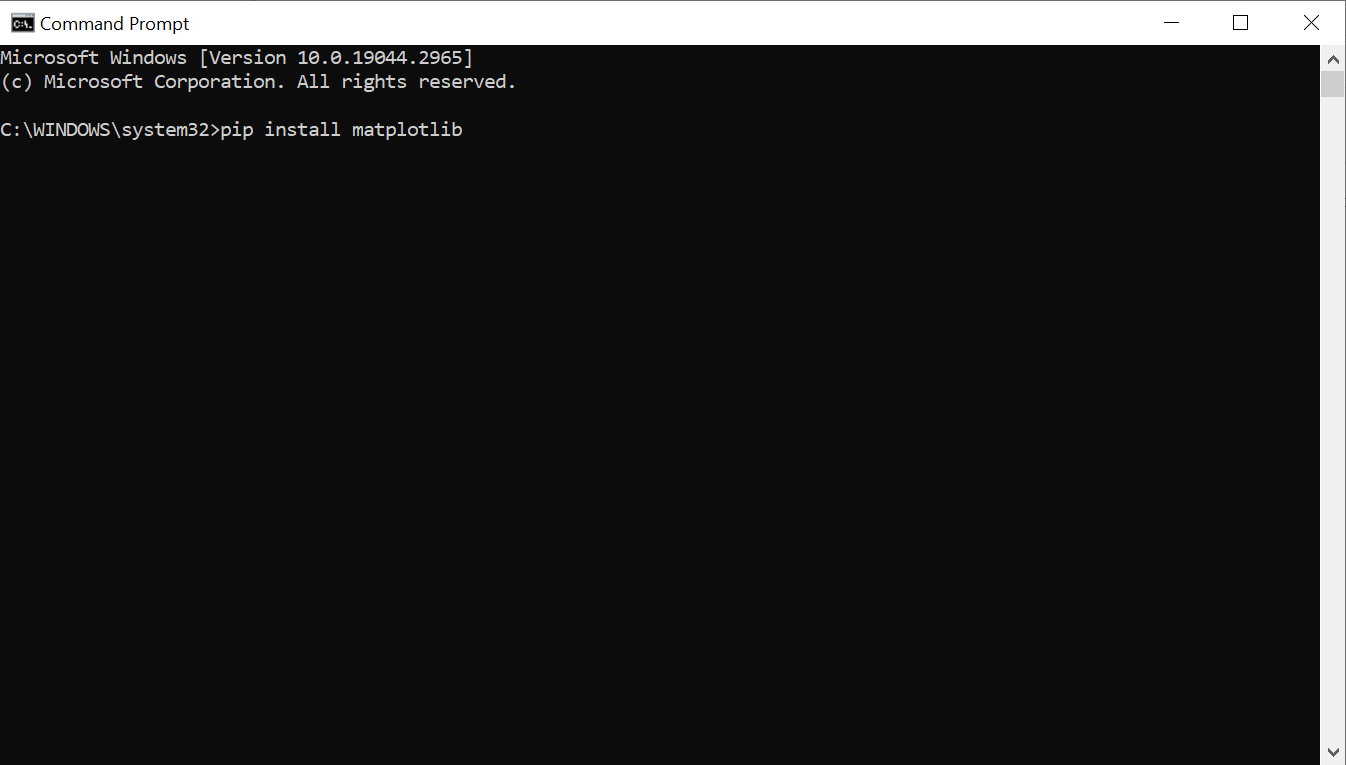
\includegraphics[width=0.8\textwidth]{Pictures/matplotlib install.png}
    \caption[Installing matplotlib]{Installing matplotlib} 
    \label{fig:part1commrin}
\end{figure}

\begin{figure}[H]
    \centering
    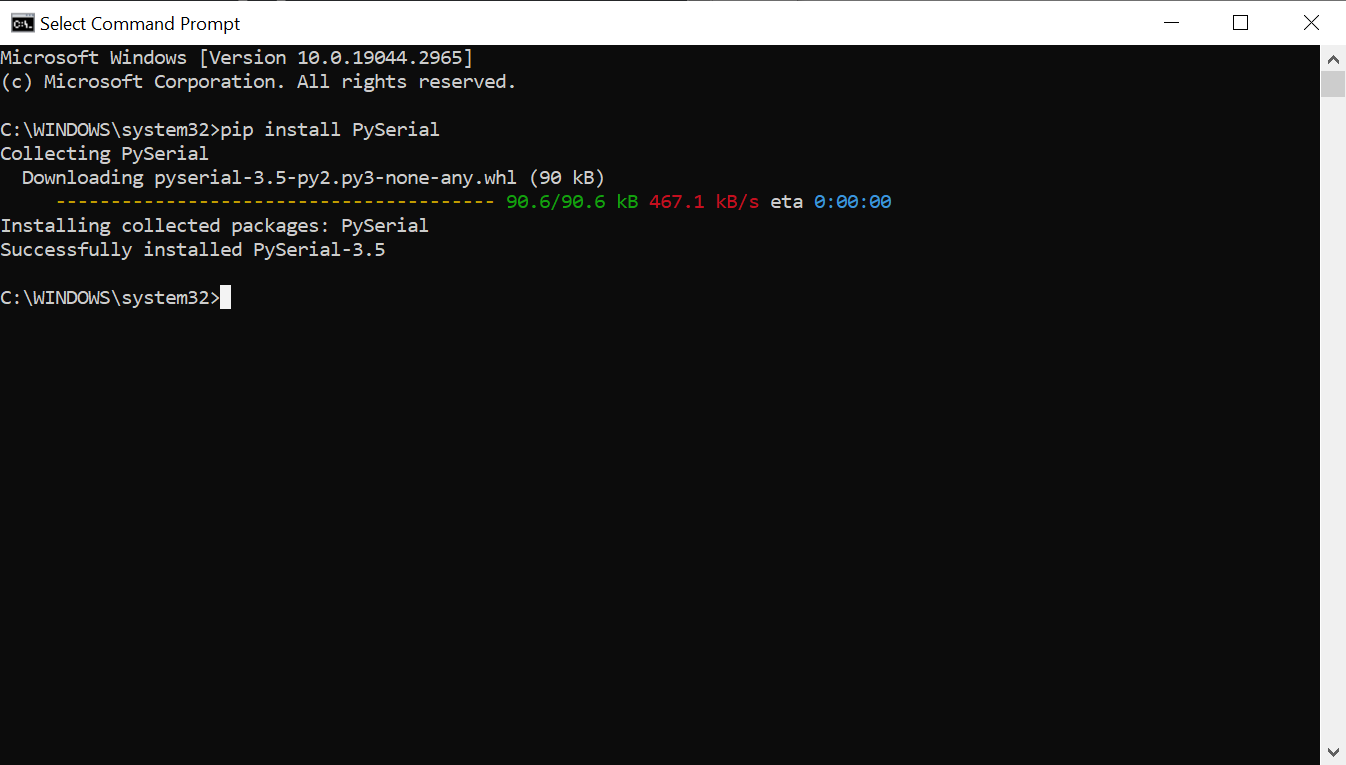
\includegraphics[width=0.8\textwidth]{Pictures/pyserial install.png}
    \caption[Installing PySerial]{Installing PySerial} 
    \label{fig:part1commrin}
\end{figure}

\item Clone or download the GitHub repository as a .zip file. If downloaded as a .zip file, extract all of its contents.

\begin{figure}[H]
    \centering
    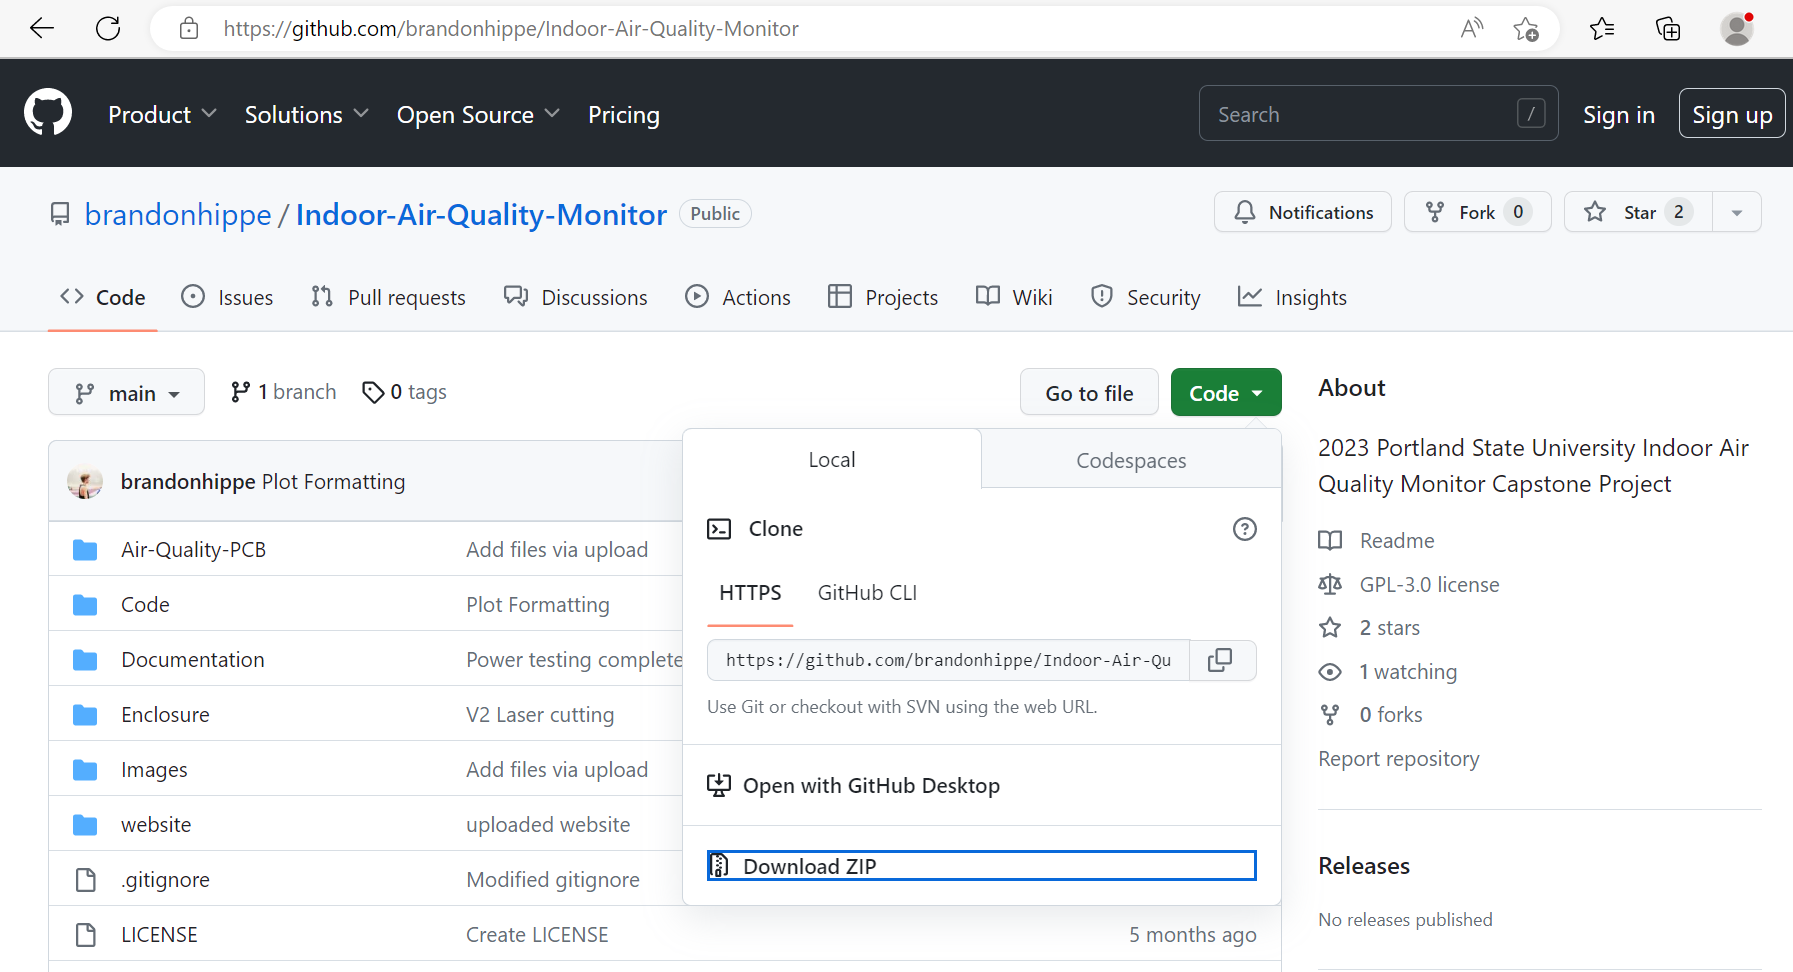
\includegraphics[width=0.8\textwidth]{Pictures/Github Download.png}
    \caption[Github Download Page]{Github Download Page} 
    \label{fig:part1commrin}
\end{figure}

\item Open Device Manager and expand the Ports drop-down. Plug the DC2274A-A manager into the computer. Four new COM ports will appear. Take note of the largest of these new ports.

\begin{figure}[H]
    \centering
    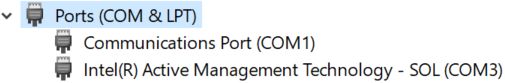
\includegraphics[width=0.8\textwidth]{Pictures/manager unplugged.png}
    \caption[Before plugging in manager]{Before plugging in manager} 
    \label{fig:part1commrin}
\end{figure}

\begin{figure}[H]
    \centering
    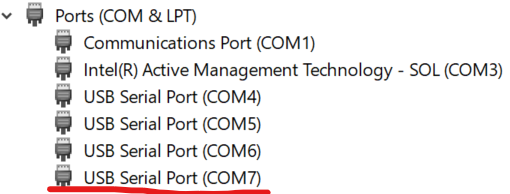
\includegraphics[width=0.8\textwidth]{Pictures/manager plugged in.png}
    \caption[After plugging in manager]{After plugging in manager. Note: 4th COM port is underlined} 
    \label{fig:part1commrin}
\end{figure}

\item Navigate to the \texttt{Code/Host Node/app/SensorDataReceiver} folder. Run the \texttt{SensorDataReceiver.py} script. In the popup window, under the port name, type in the COM port from step 3, including "COM." Click connect, and the box should turn green to indicate a successful connection.

\begin{figure}[H]
    \centering
    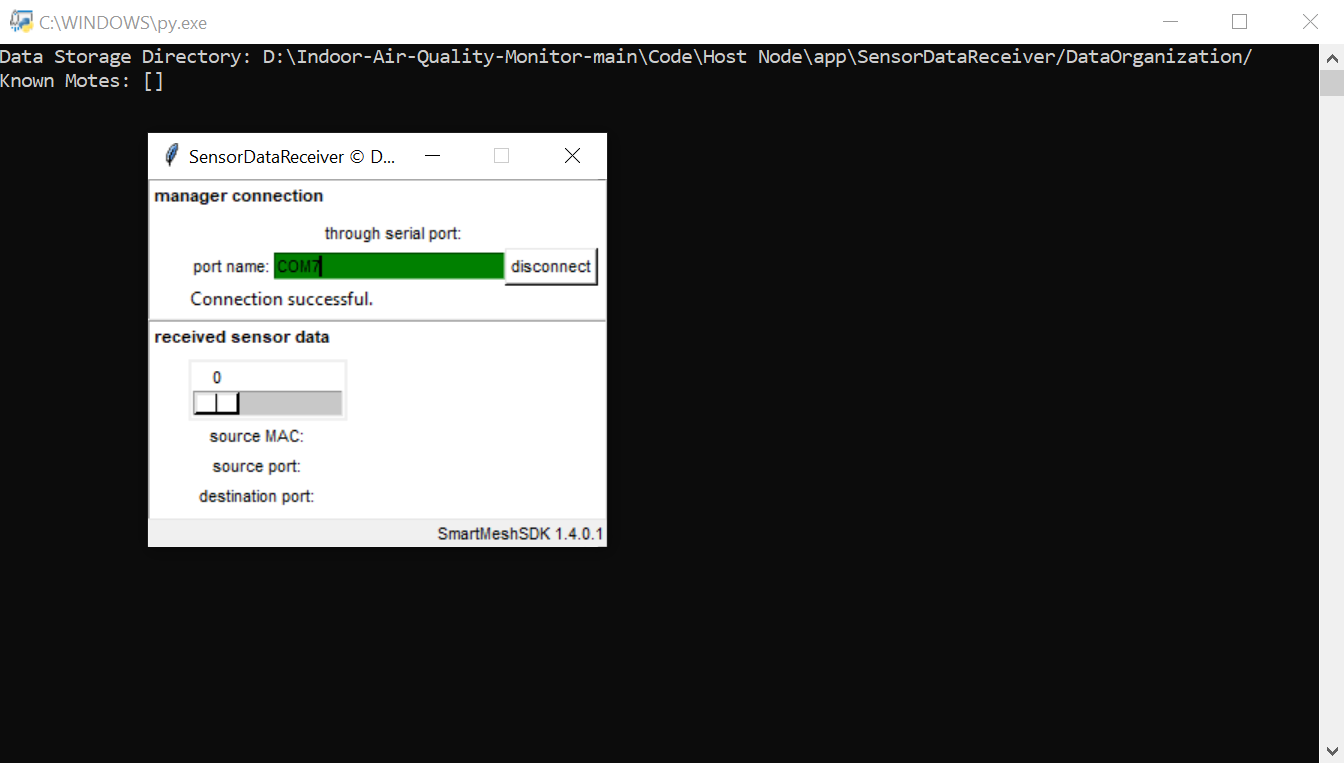
\includegraphics[width=0.8\textwidth]{Pictures/manager connected.png}
    \caption[Manager Connected]{Manager Connected} 
    \label{fig:part1commrin}
\end{figure}

\item From the same folder, run the \texttt{iaqGraphing.py} script. A window with three plots should appear on the screen. At the bottom, click the "Plot Example" button. Example data should be plotted in each of the plots.

\begin{figure}[H]
    \centering
    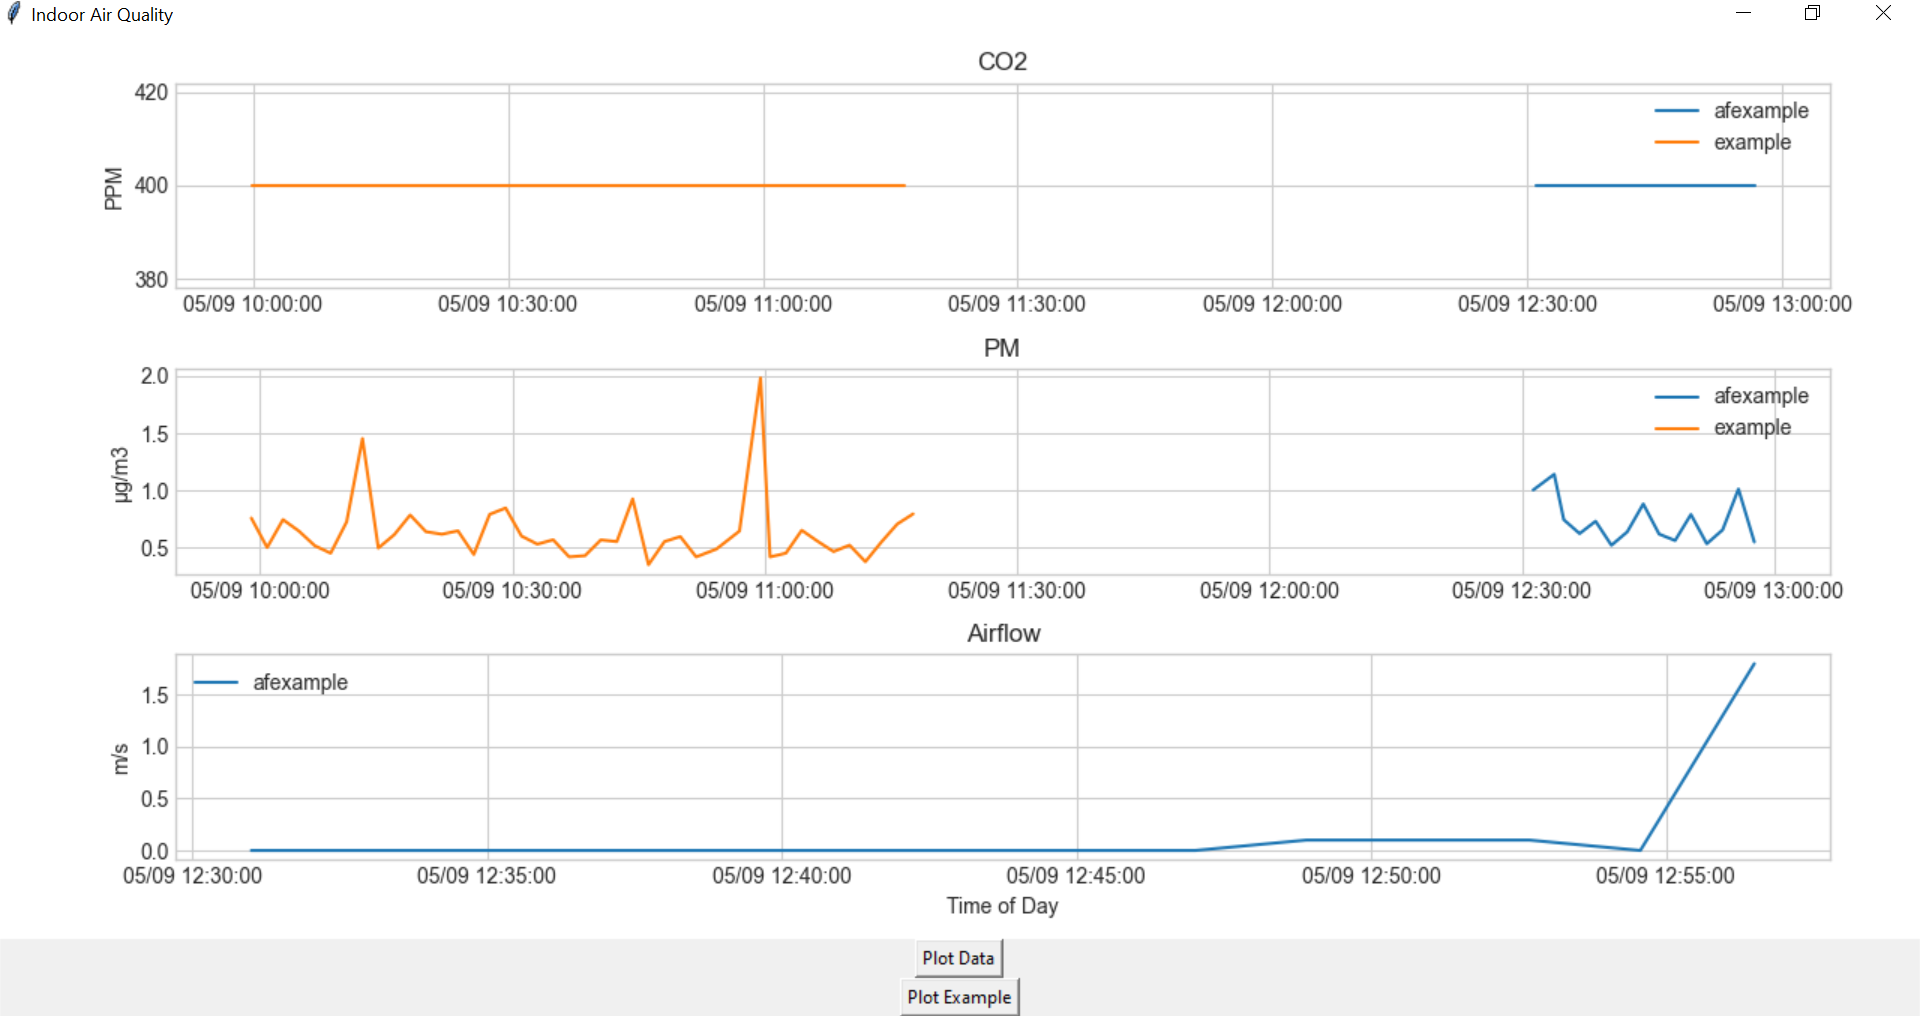
\includegraphics[width=0.8\textwidth]{Pictures/example plotted.png}
    \caption[Example data plotted]{Example data plotted} 
    \label{fig:part1commrin}
\end{figure}

\item Now click on the "Plot Data" button. The graph will now plot new data received from the sensors approximately every 10 seconds and display all the data over the last 24 hours.

\begin{figure}[H]
    \centering
    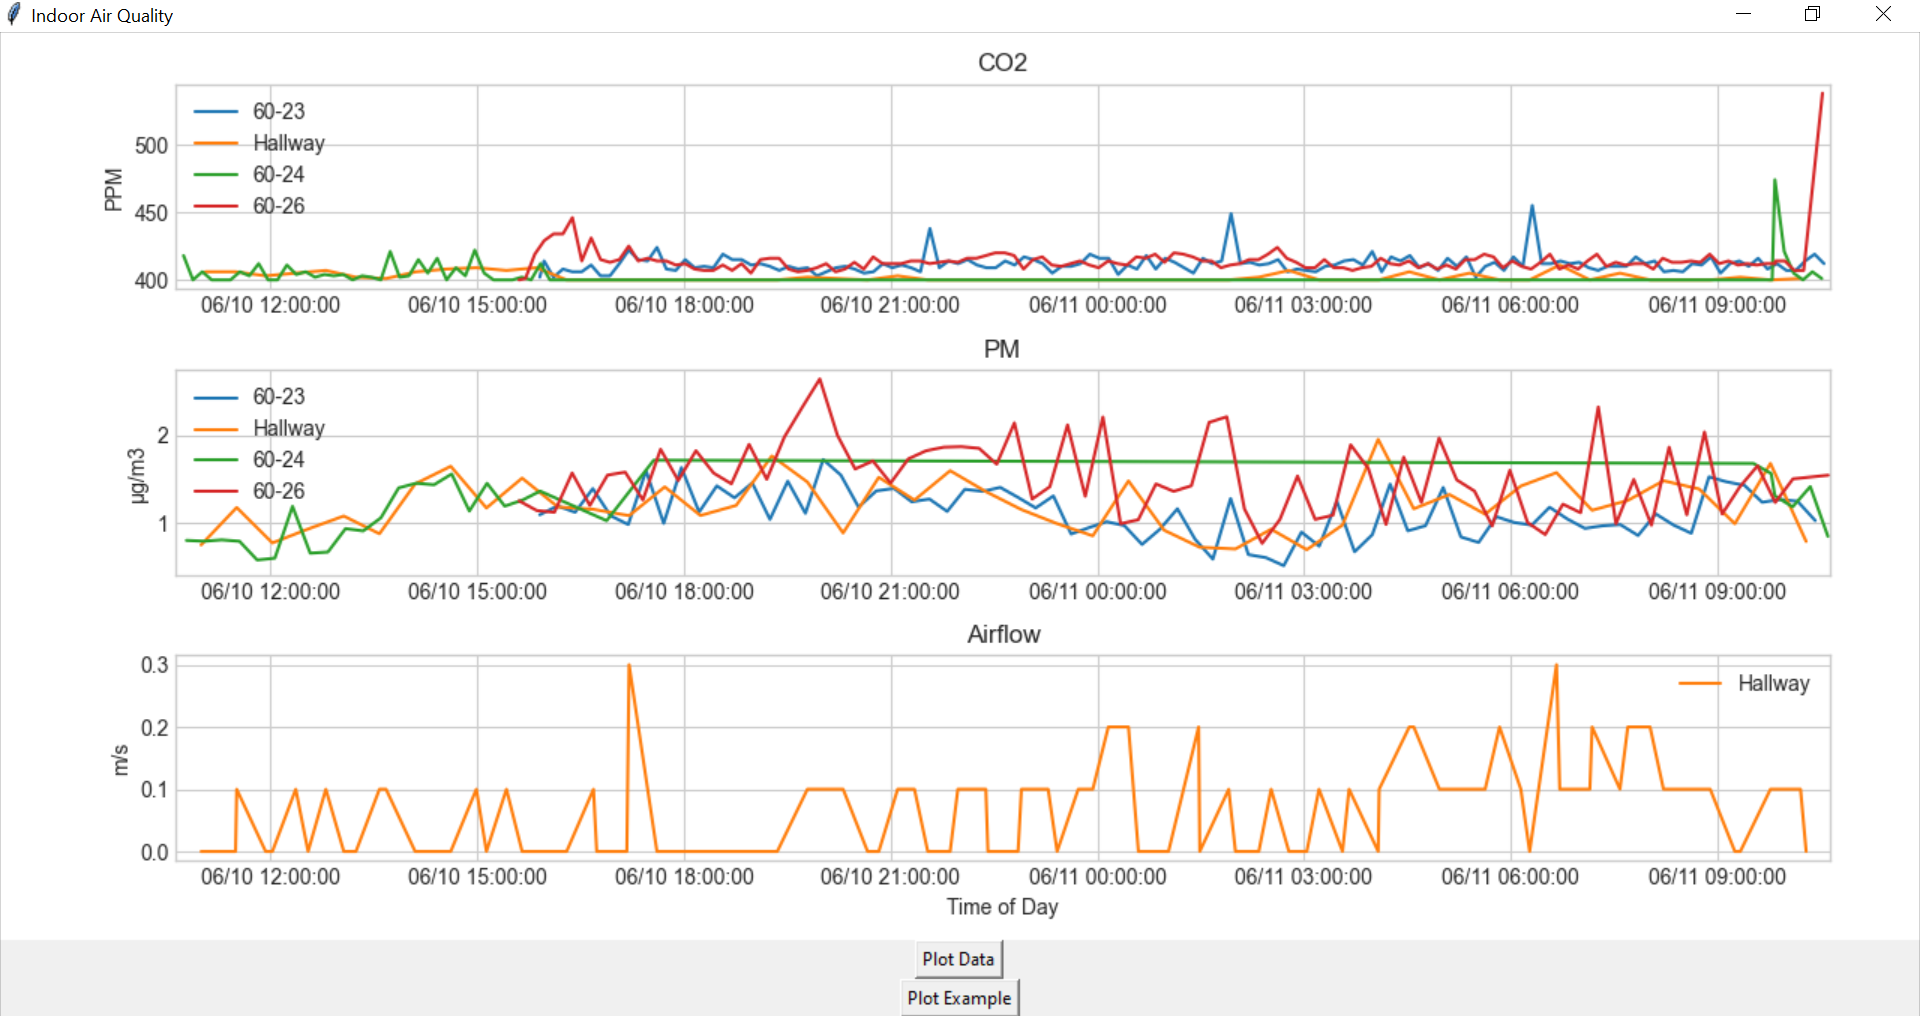
\includegraphics[width=0.8\textwidth]{Pictures/Data Plotted.png}
    \caption[Sensor Data Plotted]{Sensor Data Plotted} 
    \label{fig:part1commrin}
\end{figure}

\end{enumerate}

\subsection{Setting up Sensor Nodes}
\begin{enumerate}
\item Download Energia. Links to download as well as versions used at the time can be found in the project resources section of this report.
\item Open the \texttt{Code/Sensor Mote/libraries} folder in the downloaded repository. Copy the contents of this folder into the library folder of your Energia installation (for easiest use, move the Energia folder to the C drive, so the path is something like \texttt{C:\textbackslash energia-1.8.10E23}).

\begin{figure}[H]
    \centering
    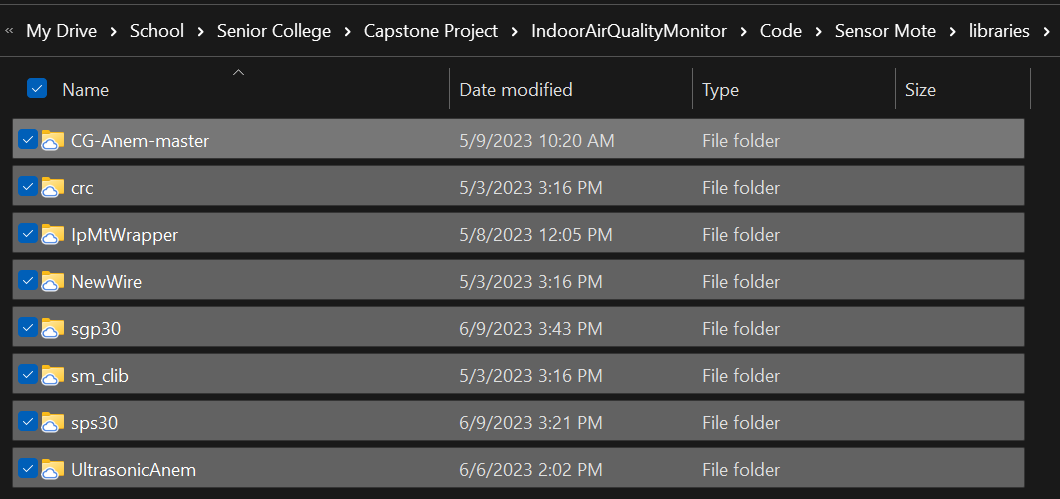
\includegraphics[width=0.8\textwidth]{Pictures/Libraries to copy.png}
    \caption[Energia libraries needed]{Energia libraries needed} 
    \label{fig:part1commrin}
\end{figure}

\begin{figure}[H]
    \centering
    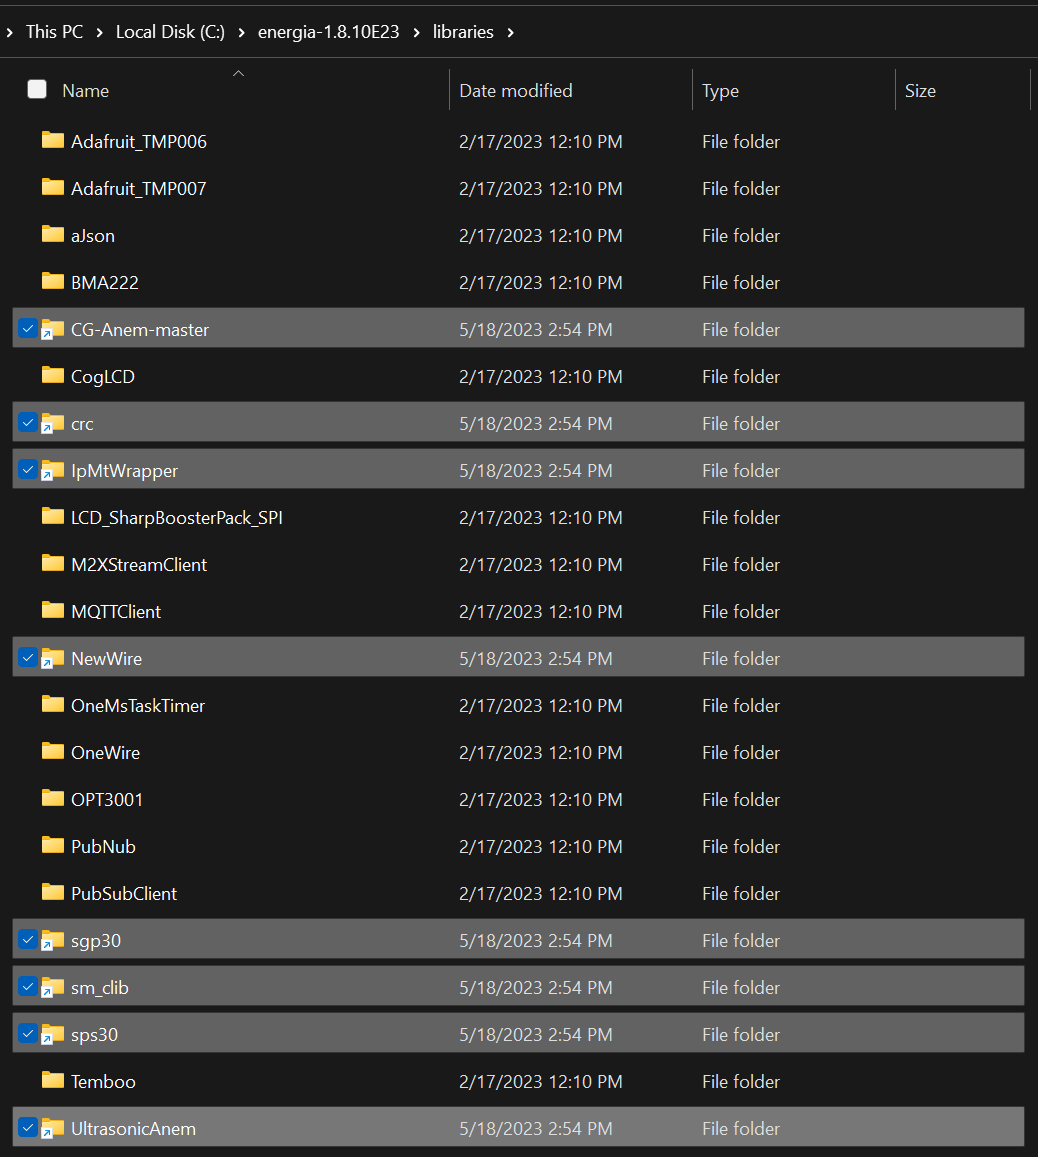
\includegraphics[width=0.8\textwidth]{Pictures/Libraries copied.png}
    \caption[Libraries copied]{Libraries copied to \texttt{C:\textbackslash energia-1.8.10E23\textbackslash libraries} folder} 
    \label{fig:part1commrin}
\end{figure}

\item Launch Energia and make sure to select the "MSP-EXP430FR2355LP" in the board section under the Tools tab.

\begin{figure}[H]
    \centering
    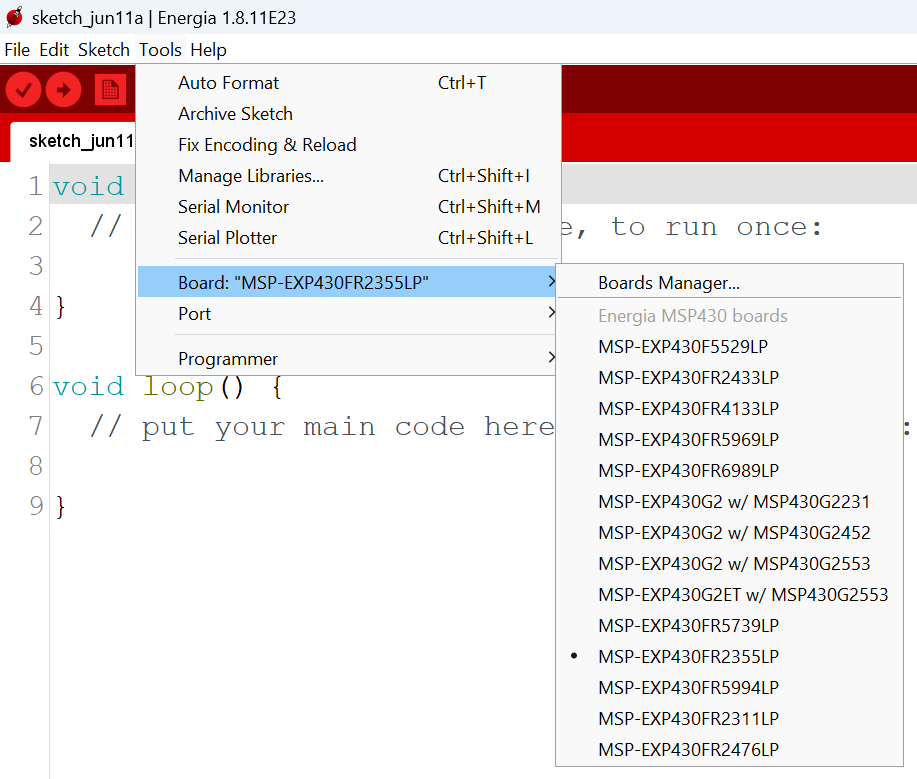
\includegraphics[width=0.8\textwidth]{Pictures/Energia Started and board selected.png}
    \caption[MSP430FR2355 Selected]{MSP430FR2355 Selected} 
    \label{fig:part1commrin}
\end{figure}

\item Under File, press open, then navigate to the downloaded repository. Navigate to \texttt{Code/Sensor Mote/indoor\_air\_quality\_v2} and open \texttt{indoor\_air\_quality\_v2.ino}.
\item Click on the red checkmark to verify the code and make sure it compiles without errors.

\begin{figure}[H]
    \centering
    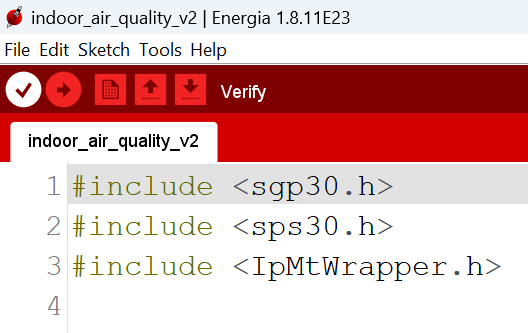
\includegraphics[width=0.8\textwidth]{Pictures/Verify Button.png}
    \caption[Verify button]{Verify button} 
    \label{fig:part1commrin}
\end{figure}

\begin{figure}[H]
    \centering
    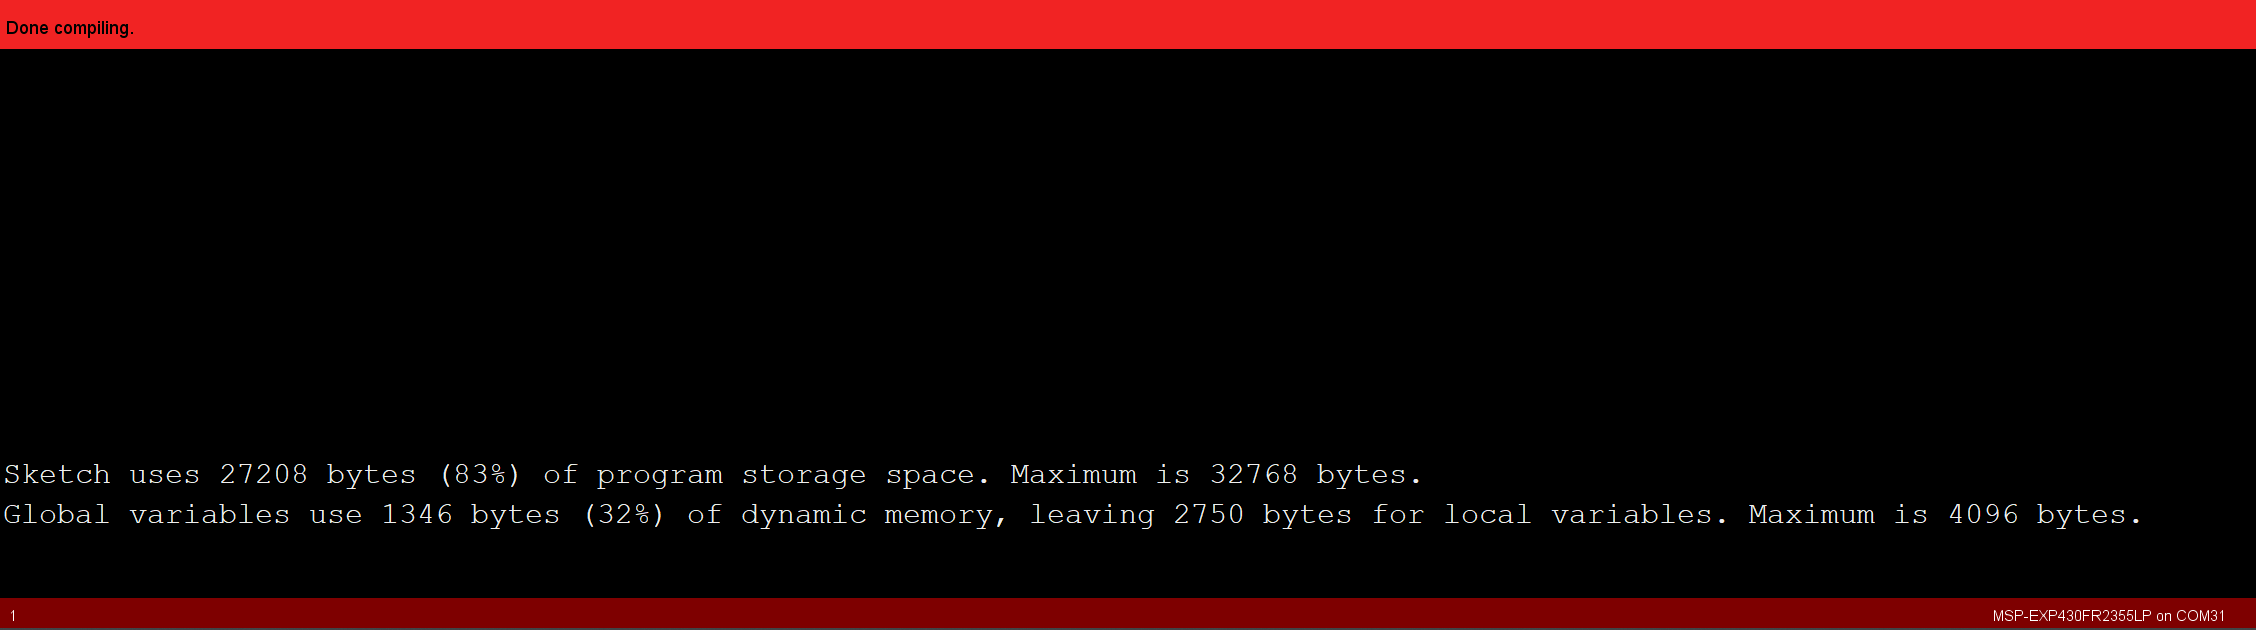
\includegraphics[width=0.8\textwidth]{Pictures/Code verified.png}
    \caption[Code compiled]{Code compiled without errors} 
    \label{fig:part1commrin}
\end{figure}

\item Remove the lid of the sensor node.
\item Plug the other end of the USB cable plugged into the MSP430 into the computer.
\item Open Device Manager and check under the Ports drop-down for a device named "MSP Application UART 1" and take note of the COM port number associated with it.

\begin{figure}[H]
    \centering
    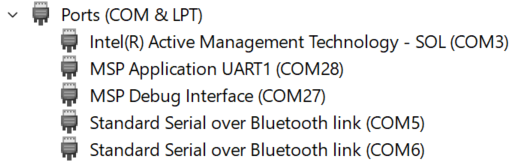
\includegraphics[width=0.8\textwidth]{Pictures/device manager.png}
    \caption[MSP430 in device manager]{MSP430 in device manager} 
    \label{fig:part1commrin}
\end{figure}

\item In Energia, select the COM port from step 10 in the Port section under the Tools tab.

\begin{figure}[H]
    \centering
    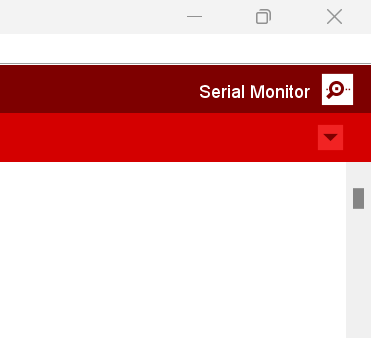
\includegraphics[width=0.8\textwidth]{Pictures/serial monitor button.png}
    \caption[Serial monitor button]{Serial monitor button} 
    \label{fig:part1commrin}
\end{figure}

\item Open the Serial Monitor by clicking on the magnifying glass in the top-right corner. Have this visible to see debug output after programming the MSP430.
\item Click the red right arrow next to the checkmark to upload the code to the MSP430.

\begin{figure}[H]
    \centering
    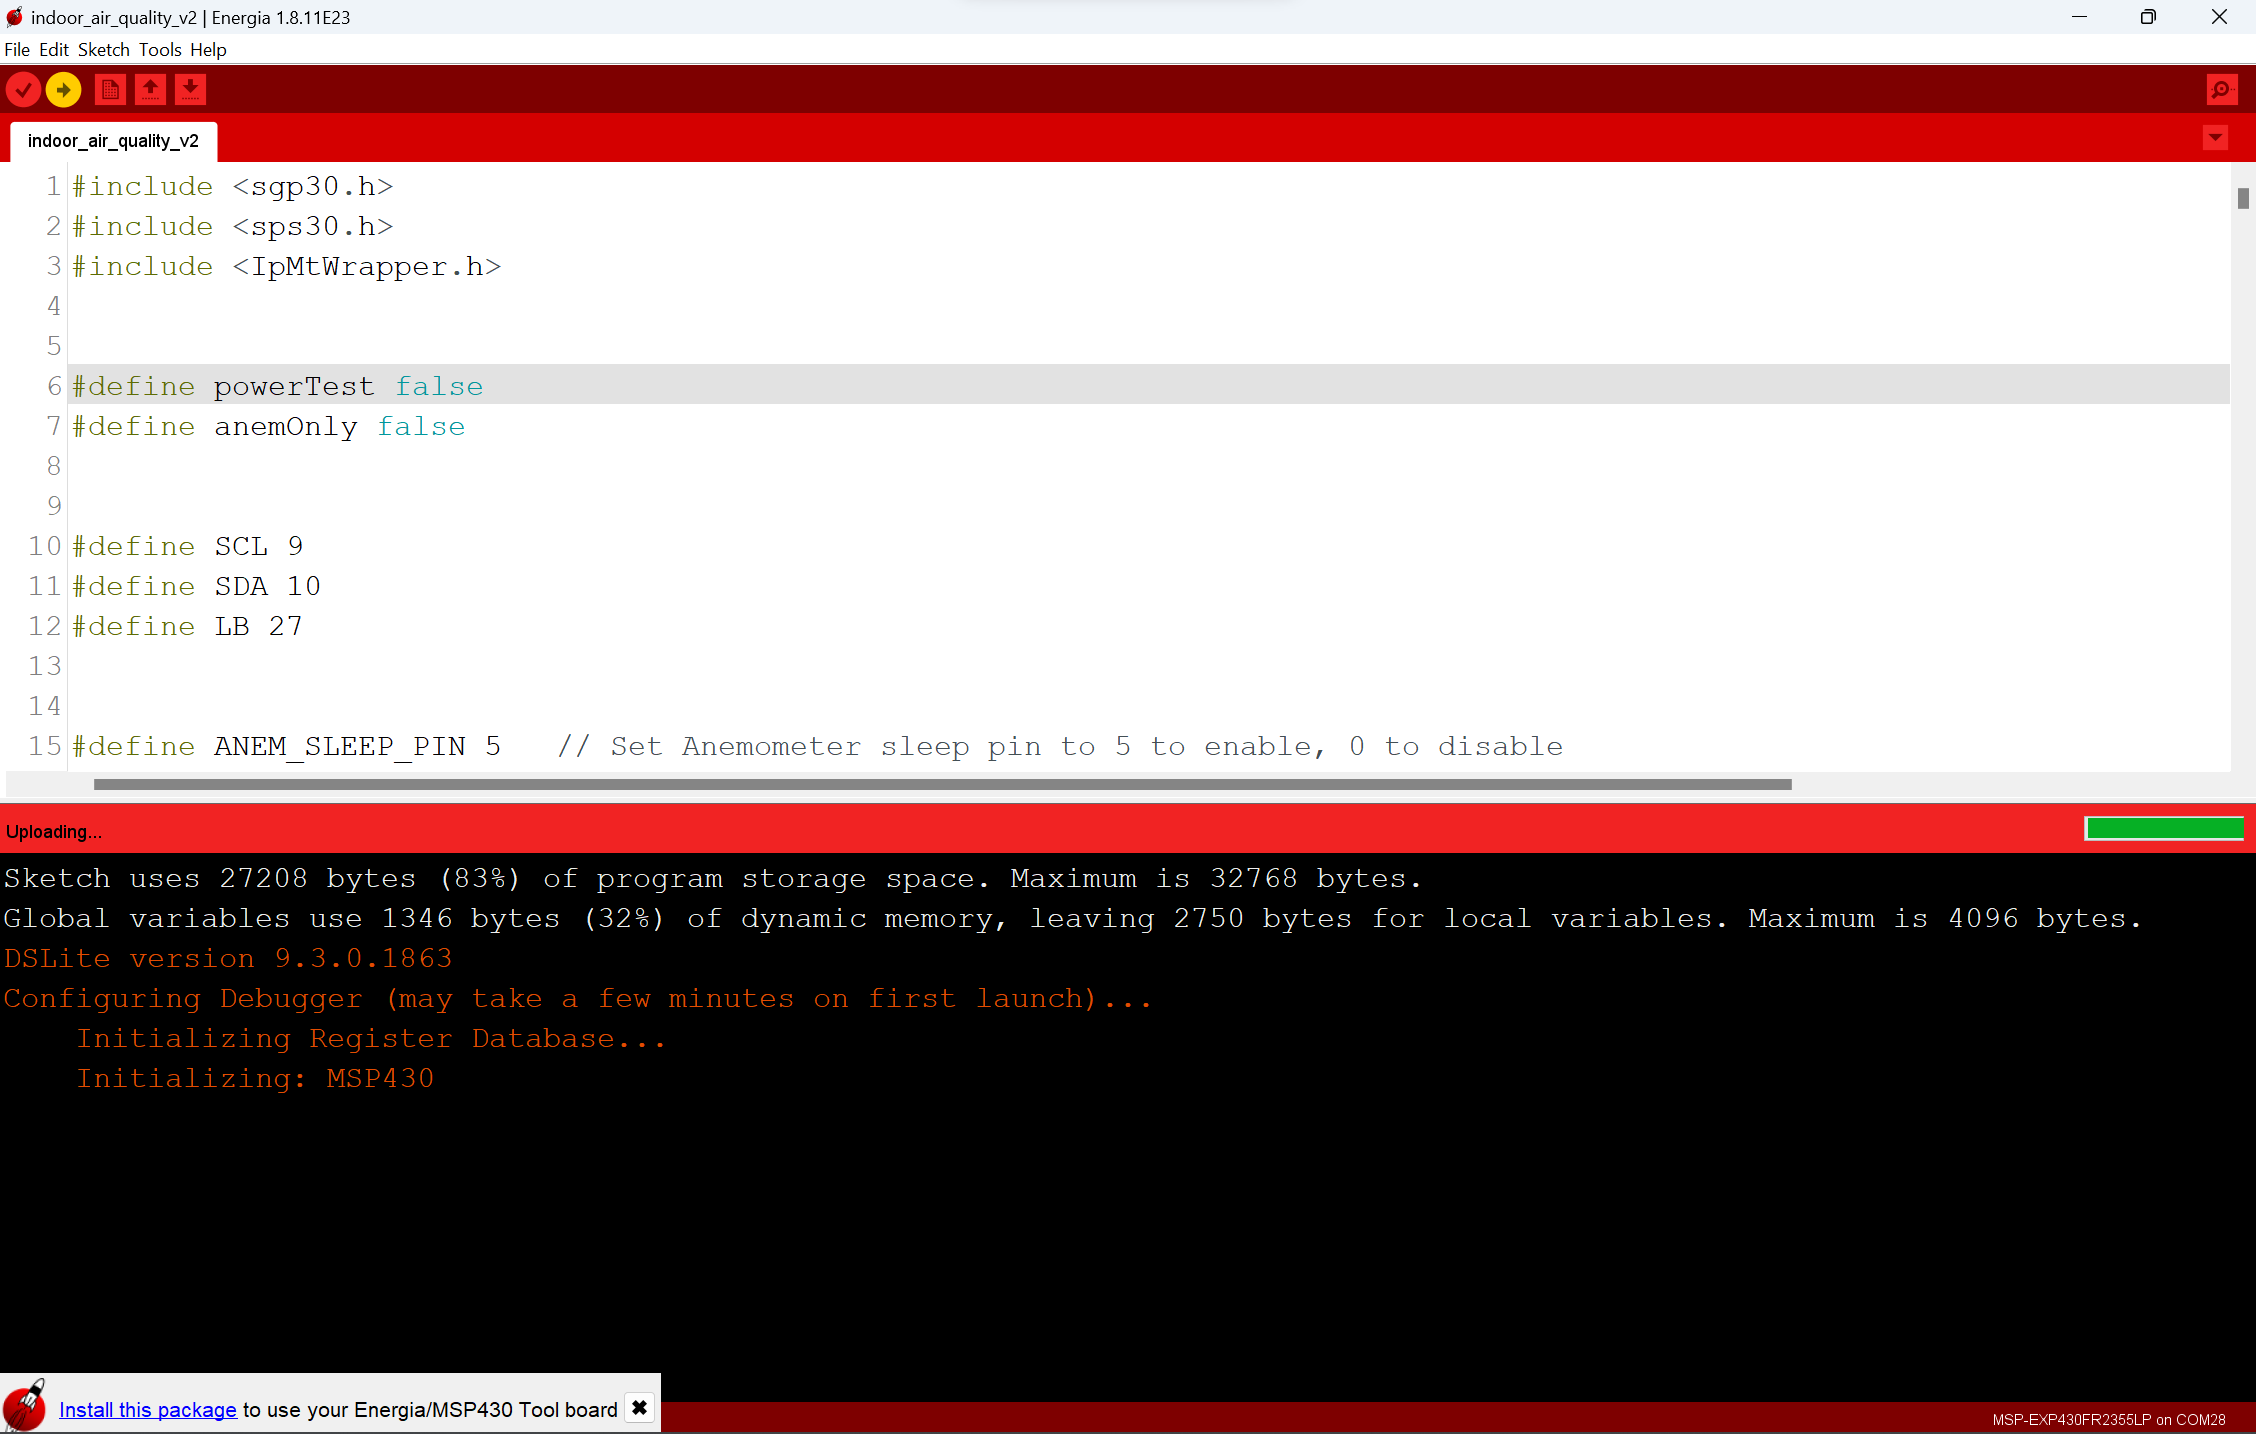
\includegraphics[width=0.8\textwidth]{Pictures/code uploading.png}
    \caption[Code uploading to MSP430]{Code uploading to MSP430} 
    \label{fig:part1commrin}
\end{figure}

\item Watch the Serial Monitor. You should see messages related to the SmartMesh system connecting to the host node. Once it connects, you'll see each of the installed sensors take their first measurements and send them to the host node.
\item On the SensorDataReceiver.py terminal, verify that the first measurements from the sensors are received. It is now safe to unplug the USB cable from the computer, place it back in the sensor node, close the sensor node, and mount the node wherever you'd like to collect indoor air quality data.

\begin{figure}[H]
    \centering
    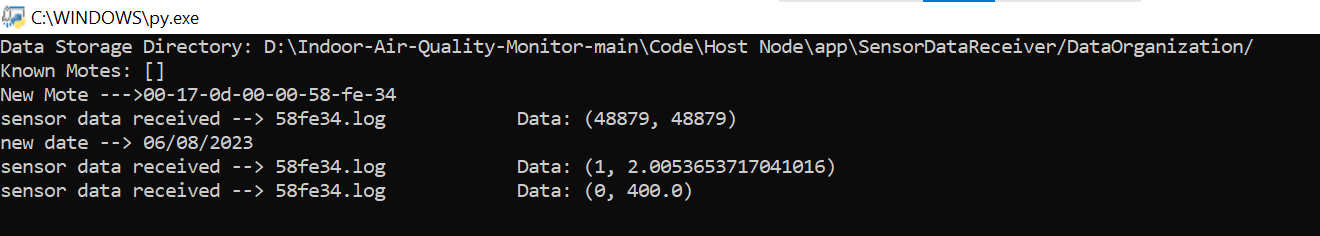
\includegraphics[width=0.8\textwidth]{Pictures/data received.png}
    \caption[Data received by host node]{Data received by host node} 
    \label{fig:part1commrin}
\end{figure}

\item Repeat steps 7-14 for any additional sensor nodes.
\end{enumerate}
